\section{Concrete agendas change native planning and accepted output}
\label{sec:native-catalog}
\subsection{Matched authority without changing production laws}
The capacity pilot protects original project selection; it does not test
whether institutions can improve that selection. We therefore conduct a
separate three-arm developer intervention, retaining the same five initial
Qwen3-8B university researchers, four native years, corpus, reserve-proximity
allocation and reused development seed 61001. All three specifications have
the same initial graph, available grants and agenda-generation rule. The
institution chooses the shortest topic in each eligible researcher's actual
displayed expertise catalog, breaking ties lexically. Only its actuation differs:
no effect, concrete advice before original planning, or direct legal assignment.
These are explicit hand-written controls, not generated discoveries.

The new catalog-assignment action must preserve the exact displayed topic,
native catalog content and duration, and can apply only to an active idle
author. It cannot shorten ongoing work or create an artificial output. This
is an explicitly named extension of institutional authority, not a weakening
of the earlier fixed-production scope or unrestricted permission to replace
native production. Original native costs, funding, submission capacity,
calendar and accounting remain operative. The shortest-topic rule is a
particular control, not a requirement imposed on generated institutions.

Every arm receives both unchanged losses $T$ and $P$. Neither is a constraint
on the other. No criterion requires advice to be obeyed, a topic to change,
or either loss to improve. All three worlds complete without replacement.
Two original-source audits and two cost projections agree; the choice, effect
and complete-input readers each export identically twice, as does the final
figure and table export. Table~\ref{tab:catalog-controls} retains all conditions.

\begin{table}[t]
\centering\small
\begin{tabular}{lrrrrr}
\toprule
Agenda actuation & T & P & Scientist replies & Planning calls & Assignments\\
\midrule
No effect & $-12$ & $-15$ & 148 & 9 & 0\\
Concrete advice & $-18$ & $-16$ & 180 & 10 & 0\\
Direct assignment & $-18$ & $-16$ & 168 & 0 & 10\\
\bottomrule
\end{tabular}
\caption{All three native planning controls at one reused development seed.
Planning calls are original research-direction requests; assignments are
catalog-validated native effects, not completed projects. Both effectful
arms improve accepted-count loss and saved-founder activity together.
This is not objective-conditioned search or independent replication.}
\label{tab:catalog-controls}
\end{table}

\subsection{Observed choices and an actual institutional consumer}
Without agenda actuation, initial projects have catalog durations
3,3,3,2,2 years. Both effectful arms start with 2,2,2,2,2-year projects and
start another two-year project for each eligible founder in year 3.
Saved native start and end dates retain these original catalog durations
(Figure~\ref{fig:catalog-projects}); no existing project is retroactively
shortened. A project visible in an inactive founder's saved state is not
thereby completed, and an assignment is not itself a publication.

In the advice arm, all ten original direction requests include their actual
actor/year agenda, and every uniquely attributed literal selected topic
matches that agenda. There are zero native assignment effects. This is
observed uptake by the fixed researcher model on this history, not an
assumption inferred from delivering a prompt. Direct assignment instead
produces ten validated native effects and zero original direction calls:
it replaces the choice rather than demonstrating researcher obedience.

\begin{figure}[t]
\centering
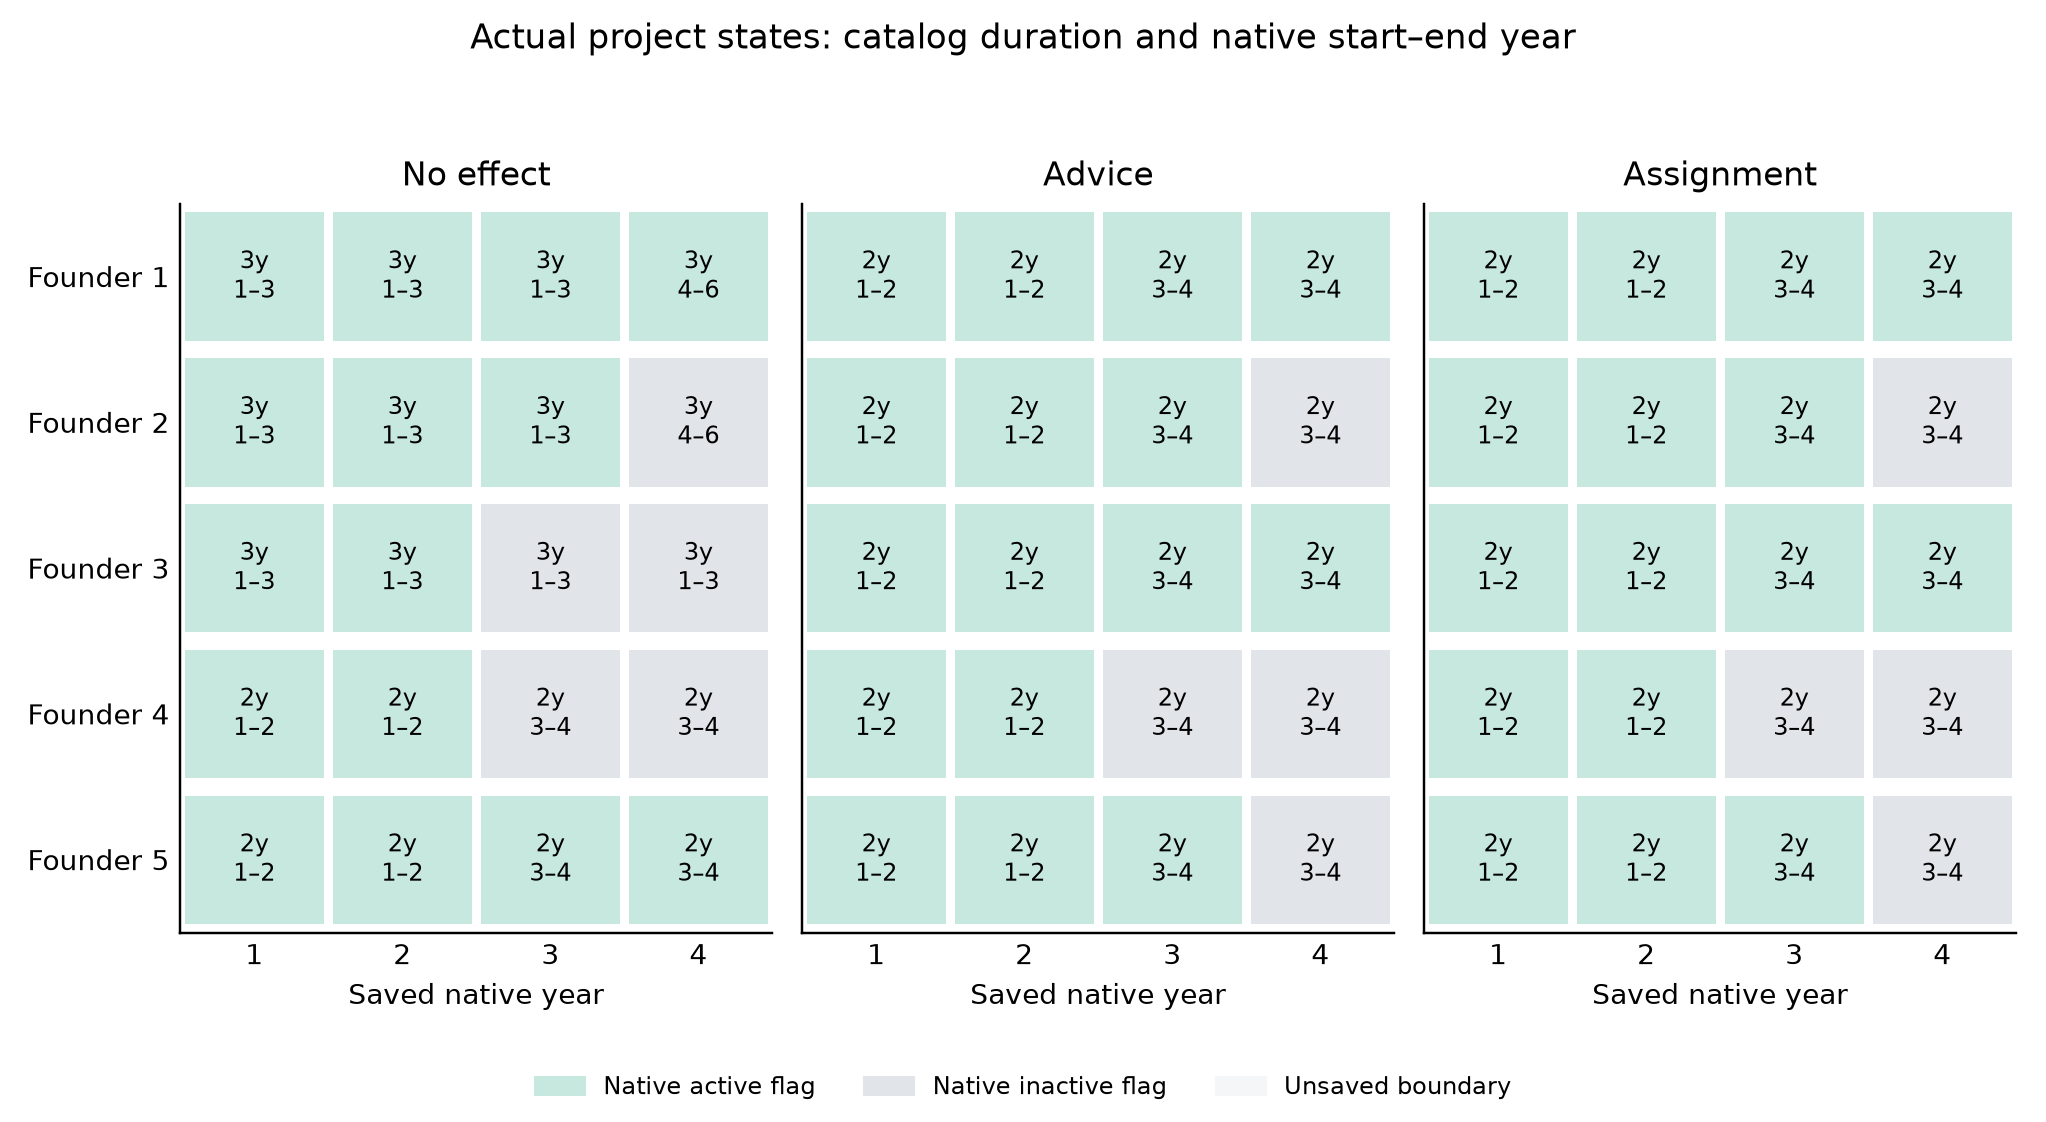
\includegraphics[width=\linewidth]{figures/native-catalog-actuation-v1/project-states.png}
\caption{Actual saved project states for all five founders and four years
in each arm. Cells show the catalog duration and native start--end years;
colors encode original active flags. Project dates and flags are different
quantities. The two-year effectful agenda contrasts with the initial mixed
two/three-year path, without changing original production laws.}
\label{fig:catalog-projects}
\end{figure}

The effectful arms each have 18 rather than 12 accepted decision records
and 16 rather than 15 active founder boundaries. Their annual active counts
are 5,5,4,2 versus 5,5,3,2 for no effect
(Figure~\ref{fig:catalog-losses}). All three end with two active founders.
Final total founder resources are 50,40,40 in the table's order, so this is
not an improvement in every reported quantity. Accepted decisions remain a
proxy, not verified discoveries; $P$ remains a native flag sum, not meaningful
work or continuous survival.

\begin{figure}[t]
\centering
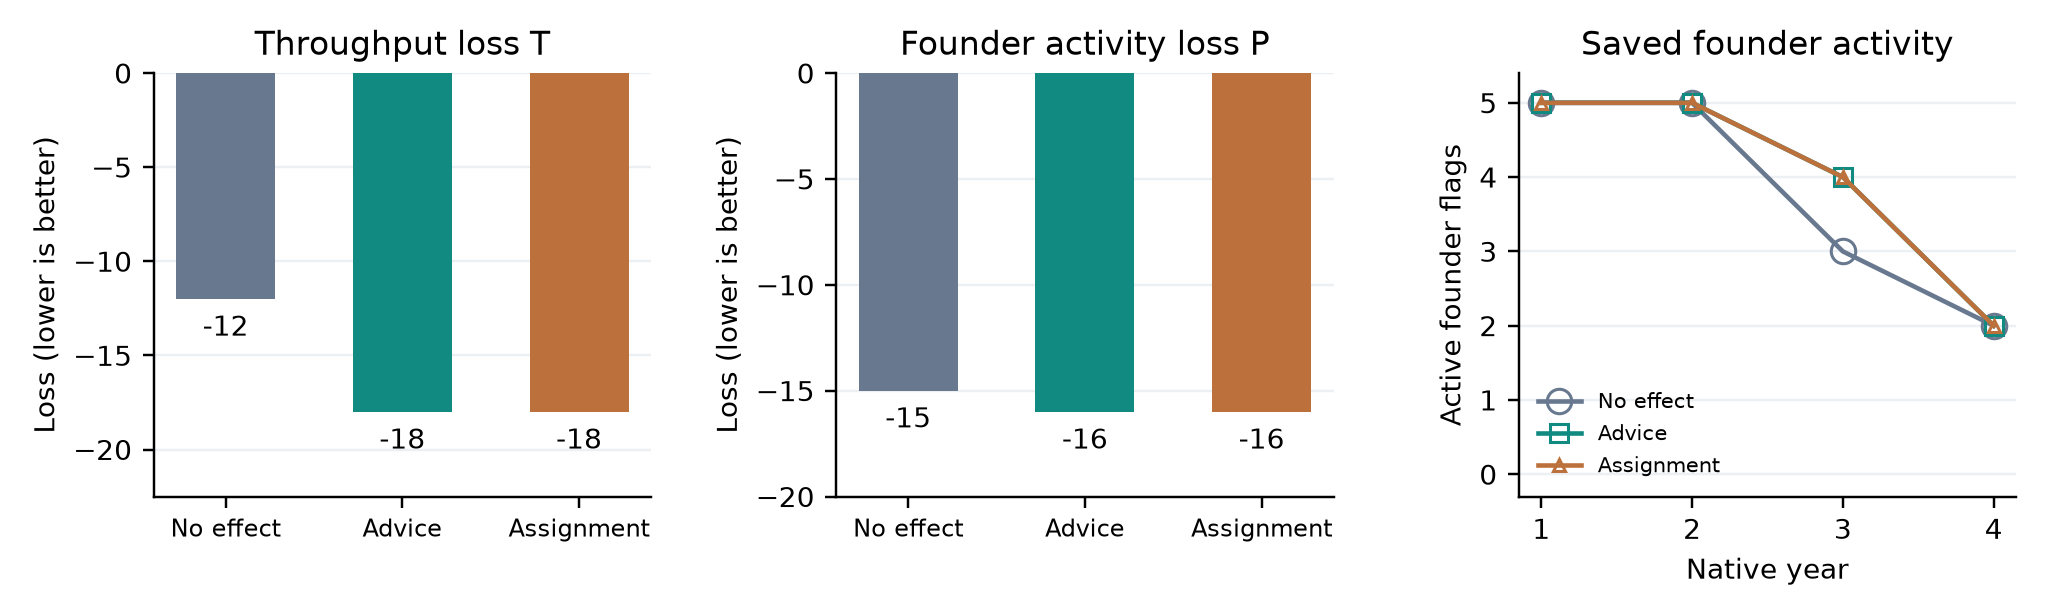
\includegraphics[width=\linewidth]{figures/native-catalog-actuation-v1/losses-and-activity.png}
\caption{Actual T/P losses and annual founder flags in all three completed
worlds. Advice and direct assignment tie both recorded losses despite distinct
request counts and full scientist-input histories. There is no observed
T/P trade-off in this comparison and no seed uncertainty estimate.}
\label{fig:catalog-losses}
\end{figure}

\subsection{Inference boundary and measured cost}
The comparison establishes an effective planning path available to an
institution, not autonomous invention or a demonstrated objective-to-system
distinction. Identical initial rules and permitted authority do not imply
identical later inputs. All three full ordered scientist-input sequences
differ, including the two equal-loss arms. Their later resource and model
response histories can evolve differently. Changed plans and accepted output
therefore do not isolate project duration as the sole mediator. The earlier
generic-advice null uses a different message and world scope; it is not a
matched message-granularity ablation of this study.

All 496 scientist requests have committed replies, with 518,946 reported
input tokens and 45,741 output tokens. The 90,562 cached prompt tokens are
a subset of input, not an additional charge. Three scientist-load POSTs have
unknown token usage. There are no designer-generation or critic POSTs.
Native execution takes 31min15s, followed by about 46s to original double
audit and cost closure. These are local observed wall times, not energy or
fresh-machine benchmarks.

This result supplies useful same-authority reference policies for subsequent
free planning/allocation search. A count/content study must still evaluate
its own actual submitted designs, both objectives and every strong reference,
then fix selections before unused-condition evaluation. A new graph is not
required; neither is a positive result. The new planning study is not counted
as complete here: its first initial-readiness attempt stops when the local
service receives a termination signal, before any reference or own candidate
world. A separately predeclared fresh attempt cannot erase that stop or its
unknown response costs. The completed three-arm evidence alone does not close
the important empirical question or justify a main-conference-ready judgment.
\FloatBarrier
